\chapter{Design and production}
In order for the next generation of DanSTAR students to be able to either replicate or improve on the current system, it is therefor important to describe how the PCB and antennas was designed and produced. This chapter will shortly clarify the design and capabilities of the telemetry PCB board in conjunction with the rest of the avionics system. Furthermore, the design and production of only the chosen antennas will be explained, these antennas are the helical antenna and the quarter-wave monopol antenna. The quarter-wave antenna was chosen, because it is easier to build and mount, than the sleeved antenna.  

\section{RICHARD}
RICHARD is short for Robust Internal Controller for High altitude Rocket Dragonfly. It is the mind of the rocket, and consists of multiple PCBs stacked upon each other. All PCB's have the same dimension but they are unique with their own functionalities. At the time of writing this thesis, RICHARD is made out of 7 board: A telemetry board, A sensor board 1, A sensor board 2, A main board, An actuator board, a power board 1 and lastly a power board 2. All of the boards are capable of communicating with each other, through CAN bus\cite{CANBus}, see figure 5.1. 

The job of the telemetry board is to relay all the data coming from the other boards, down to the ground, while also saving the data on a flash chip. Furthermore, since the telemetry board is the only board designed for RF, it also has a GPS module, used for geolocationing.

\begin{figure}[h!]
\centering
%\hspace*{-2.3cm}
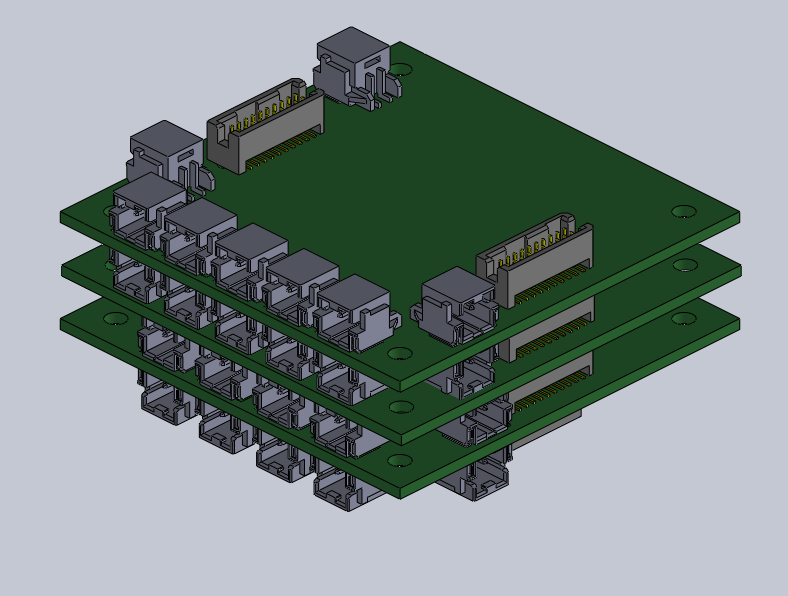
\includegraphics[scale=0.48]{figures/RICHARD.png}
\caption{A preliminary version of RICHARD, showcasing the stackable functionality}
\end{figure}

Since the telemetry system is designed to transmit data down to the ground continuously, it will a lot of power, in fact the telemetry board is the most power hungry board of all the boards, it can draw up to 1.5 - 2Amps depending on how the transceivers are configures. Since the whole stack is powered by the power board, through the side connectors, any power surges from the telemetry board can reduce the total voltage, throughout the whole stack, significantly and may introduce noise to other important IC's. That is why it is important to have a good power board, with enough power leverage, but also to use good capacitors on the telemetry board itself. The stackable design may in itself cause problems for the telemetry board, since the boards are so close to each other, the telemetry board might experience noise from the other boards, thus disturbing the sensitivity of the transceiver resulting in loses. For now it is hard to test, since RICHARD is still under development, but once it is ready a test needs to be conducted to quantify the problem. 
 
\section{PCB design}
For this section it will be out of the scope of this thesis to explain the design process of the telemetry board, but what will be explained is the specific components used in the RF section of the telemetry board, for a full overview of the design see the github link, \url{https://github.com/DanSTAR-DTU/FlightElectronicsDolken/tree/TelemetryBoard}. A PDF file containing the schematics is in the repository. Figure H.1 on appendix H, shows the schematics only for the RF section of the telemetry board. 

What can be seen on the schematics, is that the telemetry board has 4 RF modules with 4 output SMA's. The last one, (from top to bottom) is a test module, that includes a Pi-filter/matching network (just before the SMA connect, to the right) used to match the impedance with the antennas to $50\Omega$. The 4. transceiver is not really used, since the antennas used in this thesis can be matched to $50\Omega$, by physically changing the antennas. For each RF module there are 4 very important components that be found in the link budget, because the exhibit losses and gains. The 4 components are: the transceiver - NRF24l01+\cite{nrf24l01+}, the balun\cite{Balun}, the Front-end PA/LNA - RFX2401C\cite{RFX2401C} and lastly the band filter\cite{BandFilter}. The transceiver is the one that modulates and demodulates the RF signal, it it also the transceiver that the microcontroller programs. Some of the key functionalities of the transceiver are: being able to set the transmission speed (this is bound to the sensitivity too), dynamic or static payload size, error correction code, different typologies setups (point-to-point or point-to-multipoint), see also the datasheet for the the needed information\cite{nrf24l01+}. The front-end module PA/LNA, is 2-in-1 Power Amplifier and a Low Noise Amplifier, that can be set in these two states, transmit and receive mode. The purpose of the Front-end module is to amplify the signal when transmitting and increasing filtering when receiving, thus increasing the overall link margin. The Balun is used to match the output impedance of the transceiver with the input impedance of the Front-end PA/LNA module, it's a static components that does not do anything else than impedance matching. The band filter is used to filter all unwanted frequencies away, thus making the telemetry board less suitable from RF noise in different bands and from harmonic frequencies.

\begin{figure}[h!]
\centering
%\hspace*{-2.3cm}
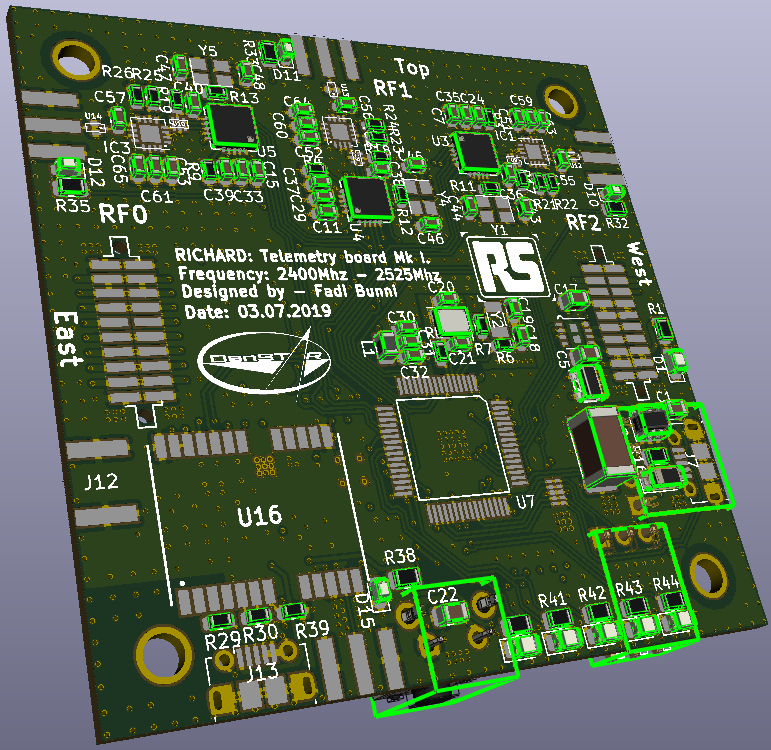
\includegraphics[scale=0.8]{figures/TelemetryBoard3D.PNG}
\caption{3-dimensional picture of the telemetry board}
\end{figure}

Figure 5.2 shows a cad model of the telemetry board. The dimension of the telemetry board is 60X60x1.6mm. Looking into the Appendix E figure E.1 in reference to figure 5.2, it is visually possible to see some of the rules been upheld, like the thermal relief rule, see figure 5.3 for all the "dots". These are called vias used to electronically connect the upper layer with bottom layer to the middle ground layer, thus reducing RF noise. They can be seen on the edge of the board too.   

Figure 5.3 shows the overview of the important section on the telemetry board. The red box the analog part while the green box is the digital part. Blue box the the flash chip, orange box is the power supply section, the yellow box is the GPS (green side not red) and lastly the gray box (a bit hard to see) is the microcontroller with its crystals. The 4 corner holes are used to fix the telemetry board together with rest of the stack (RICHARD).  

\begin{figure}[h!]
\centering
%\hspace*{-2.3cm}
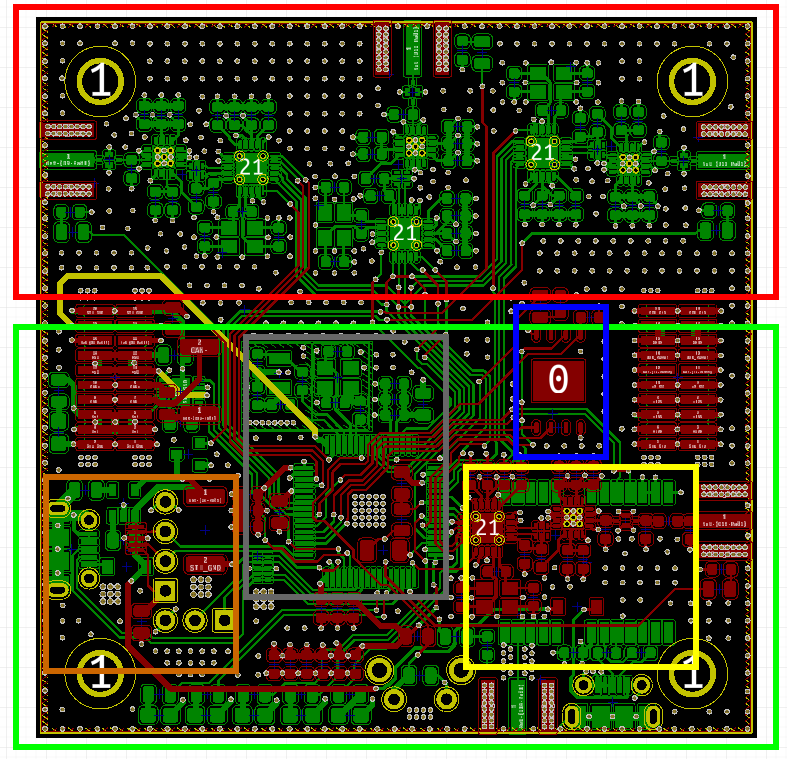
\includegraphics[scale=0.8]{figures/TelemetryBoardDesignFinished.PNG}
\caption{2-dimensional picture of the board layout - split up in important sections}
\end{figure}

\newpage

\section{Avionics compartment for antennas}

\subsection{Cad modelling}

\section{Quarter-wave monopol antenna}

\subsection{Materials}

\subsection{Construction}

\section{Helical antenna}

\subsection{Cad modelling}

\subsection{Materials}

\subsection{Construction}